\clearpage
\section{Continuous Variable QKD Transmission System}\label{sec:intro}

\begin{tcolorbox}	
\begin{tabular}{p{2.75cm} p{0.2cm} p{10.5cm}} 	
\textbf{Student Name}  &:& Daniel Pereira (2017/05/01 - )\\
\textbf{Goal}          &:& Simulation and experimental validation of a CV-QKD transmission system.\\
\textbf{Directory}              &:& sdf/cv\_system  
\end{tabular}
\end{tcolorbox}

The aim of Continuous Variable Quantum Key Distribution (CV-QKD) is to encode information in observables whose measurements take continuous values.
\par
The purpose of this study is to analyse a CV-QKD transmission system in which the information is sent in the two orthogonal quadratures of a coherent state. 

\subsection{Theoretical Analysis}

In this section we describe in depth the Continuous Variables Quantum Key Distribution (\textbf{CV-QKD}) system analysed here. The CV-QKD  system enables two parties (Alice and Bob) to share a secret key to be employed in a symmetric encryption protocol. The following CV-QKD employs discrete modulation of coherent states, resulting in the Quadrature Phase Shift Keying (\textbf{QPSK}) constellation presented in Figure~\ref{fig:QPSKconst}.
\begin{figure}[h]
\centering
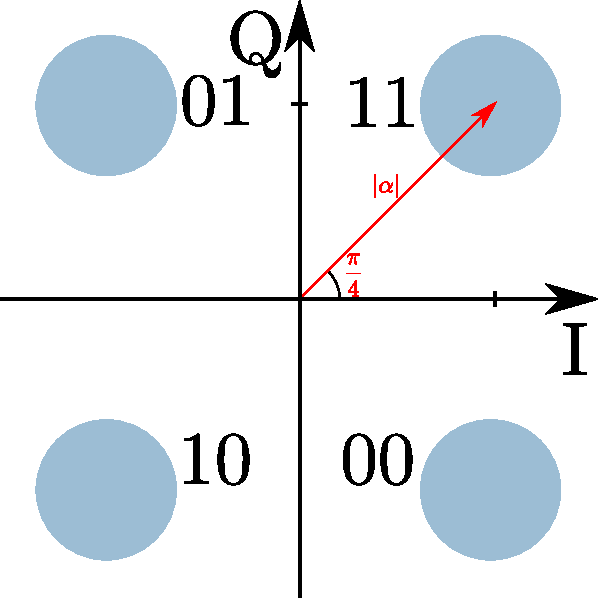
\includegraphics[width=.4\linewidth]{QPSKconstellation.pdf}
\caption{QPSK symbol constellation.}
\label{fig:QPSKconst}
\end{figure}
The state to bit correspondence, agreed by Alice and Bob beforehand, also presented in Figure~\ref{fig:QPSKconst}, is as follows:
\begin{table}[H]
\centering
\begin{tabular}{c|c}
\textbf{State} & \textbf{Bit} \\ \hline
$\ket{\alpha_0}=\ket{|\alpha|e^{i\frac{\pi}{4}}}$ & 11 \\
$\ket{\alpha_1}=\ket{|\alpha|e^{i\frac{3\pi}{4}}}$ & 01 \\
$\ket{\alpha_2}=\ket{|\alpha|e^{i\frac{5\pi}{4}}}$ & 10 \\
$\ket{\alpha_3}=\ket{|\alpha|e^{i\frac{7\pi}{4}}}$ & 00 \\
\end{tabular}
\end{table}
A step by step description of the protocol now follows:
\begin{enumerate}
\item Alice generates a random bit string of length $2N$. Lets assume that $N=8$ and that the following random bit string of length $2N=16$ is generated:
\begin{equation*}
B_\text{A}=\lbrace1,~1,~0,~1,~1,~0,~0,~1,~1,~1,~0,~1,~0,~0,~1,~0\rbrace,
\end{equation*}
\item Next, Alice sends to Bob a sequence of $N$ quantum states based on the bit string $B_\text{A}$, according to the encoding presented before, resulting in the following state sequence:
\begin{equation*}
S_\text{A}=\lbrace\ket{\alpha_0},~\ket{\alpha_1},\ket{\alpha_2},~\ket{\alpha_1},~\ket{\alpha_0},~\ket{\alpha_1},~\ket{\alpha_3},~\ket{\alpha_2}\rbrace.
\end{equation*}
\item Bob measures both quadratures of the received states and obtains two results $I_i$ and $Q_i$, $i\in1,...,N$, corresponding to the in-phase and in-quadrature components, respectively, of the $i$-th coherent state. Bob's results $b$ are related to Alice's originally encoded states $a$ by:
\begin{equation*}
b=ta+z,
\end{equation*}
which are normal linear models parametrized by $t=\sqrt{\frac{T}{2}}$ and where $z$ are the total noise contribution following a normal distribution with null mean and variance $\sigma^2$. Alice's sent states $a$ are a Bernoulli random variable taking the values $\pm\sqrt{2}|\alpha|$. 
\item Bob shares a subset of $k$ measurement results with Alice, who uses the previous linear relations to estimate the transmission channel parameters as follows:
\begin{equation*}
\tilde{t}=\frac{\sum^k_{i=1}b_ia_i}{\sum^k_{i=1}a_i^2},~\tilde{\sigma}^2=\frac{1}{k}\sum^k_{i=1}(b_i-\tilde{t}a_i)^2
\end{equation*}
These values are used to evaluate the key's security. If it is deemed not to be secure, the protocol is aborted, otherwise it continues as follows.
\item Bob attributes each measurement result to the closest corresponding possible state sent Alice, taking the considered QPSK constellation this corresponds to:
\begin{table}[H]
\centering
\begin{tabular}{c|c}
\textbf{Measurement} & \textbf{Decoded state} \\ \hline
$I_i>0~\&~Q_i>0$ & $\ket{\alpha_0}$ \\
$I_i<0~\&~Q_i>0$ & $\ket{\alpha_1}$ \\
$I_i<0~\&~Q_i<0$ & $\ket{\alpha_2}$ \\
$I_i>0~\&~Q_i<0$ & $\ket{\alpha_3}$
\end{tabular}
\end{table}
and builds a bit string according to both the measurement results and the previously agreed upon state to bit correspondence. Lets assume that Bob builds the following decoded state sequence:
\begin{equation*}
S_\text{B}=\lbrace\ket{\alpha_0},~\underline{\ket{\alpha_0}},\ket{\alpha_2},~\ket{\alpha_1},~\ket{\alpha_0},~\underline{\ket{\alpha_2}},~\underline{\ket{\alpha_2}},~\ket{\alpha_2}\rbrace,
\end{equation*}
with the corresponding bit string:
\begin{equation*}
B_\text{B}=\lbrace1,~1,~\underline{1},~1,~1,~0,~0,~1,~1,~1,~\underline{1},~\underline{0},~\underline{1},~0,~1,~0\rbrace.
\end{equation*}
The mistakes in both the bit string and state sequence are underlined.
\end{enumerate}



%The security of QKD is a complex topic to tackle, given the difficulty of proving the non-existence of an attack that cracks a protocol's security. This topic is usually approached by analysing various eavesdropping strategies and evaluating their effects on the key rate referenced in~\eqref{eq:keyrateperfect}. Information between Alice and Bob needs to be shared with current existing technology, so their shared information is always classical and Shannon's formalism is enough to describe it. However, Eve has no such restriction, so the information she has on Bob's results needs to be described according to the quantum properties of the system. 

\subsection{Simulation Analysis}

\begin{figure}[h]
\centering
%left bottom right top
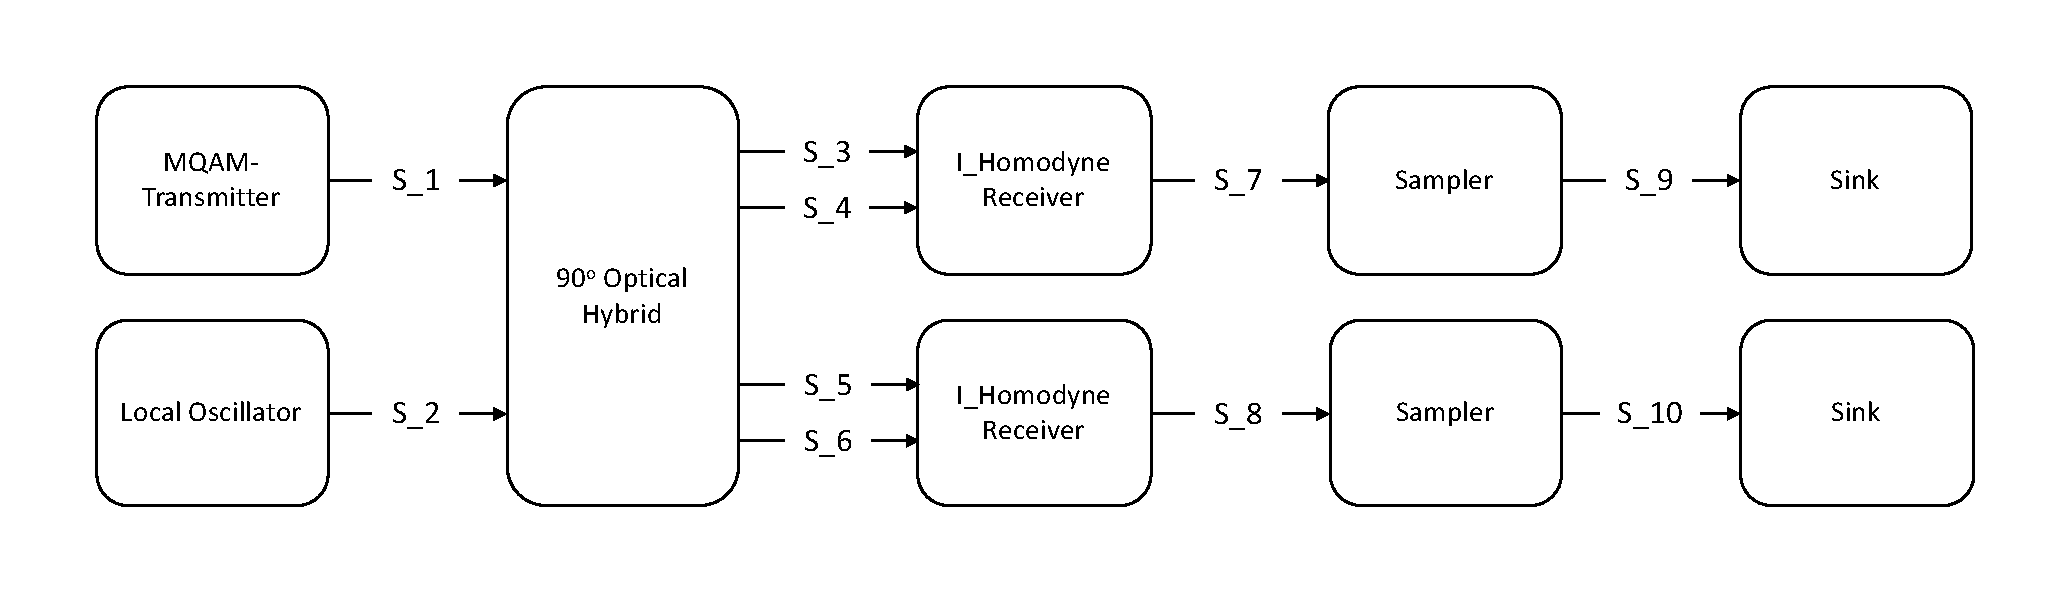
\includegraphics[width=\linewidth]{diagramSIMU.pdf}
\caption{Overview of the CV-QKD system being simulated.}
\label{fig:CV-System}
\end{figure}

\subsection*{Required files}\label{Required files}

\begin{table}[H]
\centering
\begin{tabulary}{1.0\textwidth}{|p{6cm}|p{8cm}|p{1cm}|}
\hline
\multicolumn{3}{|c|}{ \textbf{Header Files} } \\
\hline
\textbf{File}                    & \textbf{Comments} & \textbf{Status} \\ \hline
add.h                            &                   & \checkmark \\ \hline
binary\_source.h                 &                   & \checkmark \\ \hline
discrete\_to\_continuous\_time.h &                   & \checkmark \\ \hline
i\_homodyne\_reciever.h          &                   & \checkmark \\ \hline
ideal\_amplififer.h              &                   & \checkmark \\ \hline
iq\_modulator.h                  &                   & \checkmark \\ \hline
local\_oscillator.h              &                   & \checkmark \\ \hline
m\_qam\_mapper.h                 &                   & \checkmark \\ \hline
m\_qam\_transmitter.h            &                   & \checkmark \\ \hline
netxpto.h                        &                   & \checkmark \\ \hline
optical\_hybrid.h                &                   & \checkmark \\ \hline
photodiode.h                     &                   & \checkmark \\ \hline
pulse\_shaper.h                  &                   & \checkmark \\ \hline
sampler.h                        &                   & \checkmark \\ \hline
sink.h                           &                   & \checkmark \\ \hline
super\_block\_interface.h        &                   & \checkmark \\ \hline
white\_noise.h                   &                   & \checkmark \\ \hline
\end{tabulary}
\end{table}		
%
\begin{table}[H]
\centering
\begin{tabulary}{1.0\textwidth}{|p{6cm}|p{8cm}|p{1cm}|}
\hline
\multicolumn{3}{|c|}{ \textbf{Source Files} } \\
\hline
\textbf{File}                      & \textbf{Comments} & \textbf{Status} \\ \hline
add.cpp                            &                   & \checkmark \\ \hline
binary\_source.cpp                 &                   & \checkmark \\ \hline
discrete\_to\_continuous\_time.cpp &                   & \checkmark \\ \hline
i\_homodyne\_reciever.cpp          &                   & \checkmark \\ \hline
ideal\_amplififer.cpp              &                   & \checkmark \\ \hline
iq\_modulator.cpp                  &                   & \checkmark \\ \hline
local\_oscillator.cpp              &                   & \checkmark \\ \hline
m\_qam\_mapper.cpp                 &                   & \checkmark \\ \hline
m\_qam\_transmitter.cpp            &                   & \checkmark \\ \hline
netxpto.cpp                        &                   & \checkmark \\ \hline
optical\_hybrid.cpp                &                   & \checkmark \\ \hline
photodiode.cpp                     &                   & \checkmark \\ \hline
pulse\_shaper.cpp                  &                   & \checkmark \\ \hline
sampler.cpp                        &                   & \checkmark \\ \hline
sink.cpp                           &                   & \checkmark \\ \hline
super\_block\_interface.cpp        &                   & \checkmark \\ \hline
white\_noise.cpp                   &                   & \checkmark \\ \hline
\end{tabulary}
\end{table}		

\subsection*{System Input Parameters}

This system takes into account the following input parameters:

\begin{table}[H]
\centering
\begin{tabulary}{1.0\textwidth}{|p{6cm}|p{4cm}|p{5cm}|}
\hline
\multicolumn{3}{|c|}{ \textbf{System Input Parameters} } \\
\hline
\textbf{Parameter}     & \textbf{Default Value}                                     & \textbf{Comments} \\ \hline
numberOfBitsGenerated  & $40000$	                                                   &                     \\ \hline
bitPeriod              & $20\times10^{-12}$                                         &\\ \hline
samplesPerSymbol       & $16$                                                       &\\ \hline
pLength                & $5$                                                        &\\ \hline
iqAmplitudesValues     & $\lbrace~\lbrace-1,~0\rbrace~,~\lbrace1,~0\rbrace~\rbrace$ & \\ \hline
outOpticalPower\_dBm   & Variable                                                   & Value varied for presented study\\ \hline
loOutOpticalPower\_dBm & $0$                                                        & \\ \hline
localOscillatorPhase   & $0$                                                        & \\ \hline
transferMatrix         & $\lbrace~\lbrace \frac{1}{\sqrt{2}},~\frac{1}{\sqrt{2}},~\frac{1}{\sqrt{2}},~\frac{-1}{\sqrt{2}} \rbrace~\rbrace$ & \\ \hline
responsivity           & $1$                                                        & \\ \hline
amplification          & $10^3$                                                     & \\ \hline
noiseSpectralDensity   & $5\times10^{-4}\sqrt{2}$~V$^2$                             & \\ \hline
confidence             & $0.95$                                                     & \\ \hline
midReportSize          & $0$                                                        & \\ \hline
\end{tabulary}
\end{table}		

\subsection*{Inputs}

This system takes no inputs.

\subsection*{Outputs}

This system outputs the following objects:
\begin{itemize}
\item Signals:
\begin{itemize}
\item Optical Signal with coded Binary String; (S$_{1}$)
\item Local Oscillator Optical Signal; (S$_{2}$)
\item 90$^\text{o}$ Optical Hybrid Outputs; (S$_{3}$, S$_{4}$, S$_{5}$, S$_{6}$)
\item Homodyne Detectors' Electrical Output; (S$_{7}$, S$_{8}$)
\item Sampled Signals; (S$_{9}$, S$_{10}$)
\end{itemize}
\end{itemize}


\subsection{Experimental Analysis}

The main experimental setup used is presented in Figure~\ref{fig:expDia}.
\begin{figure}[H]
\centering
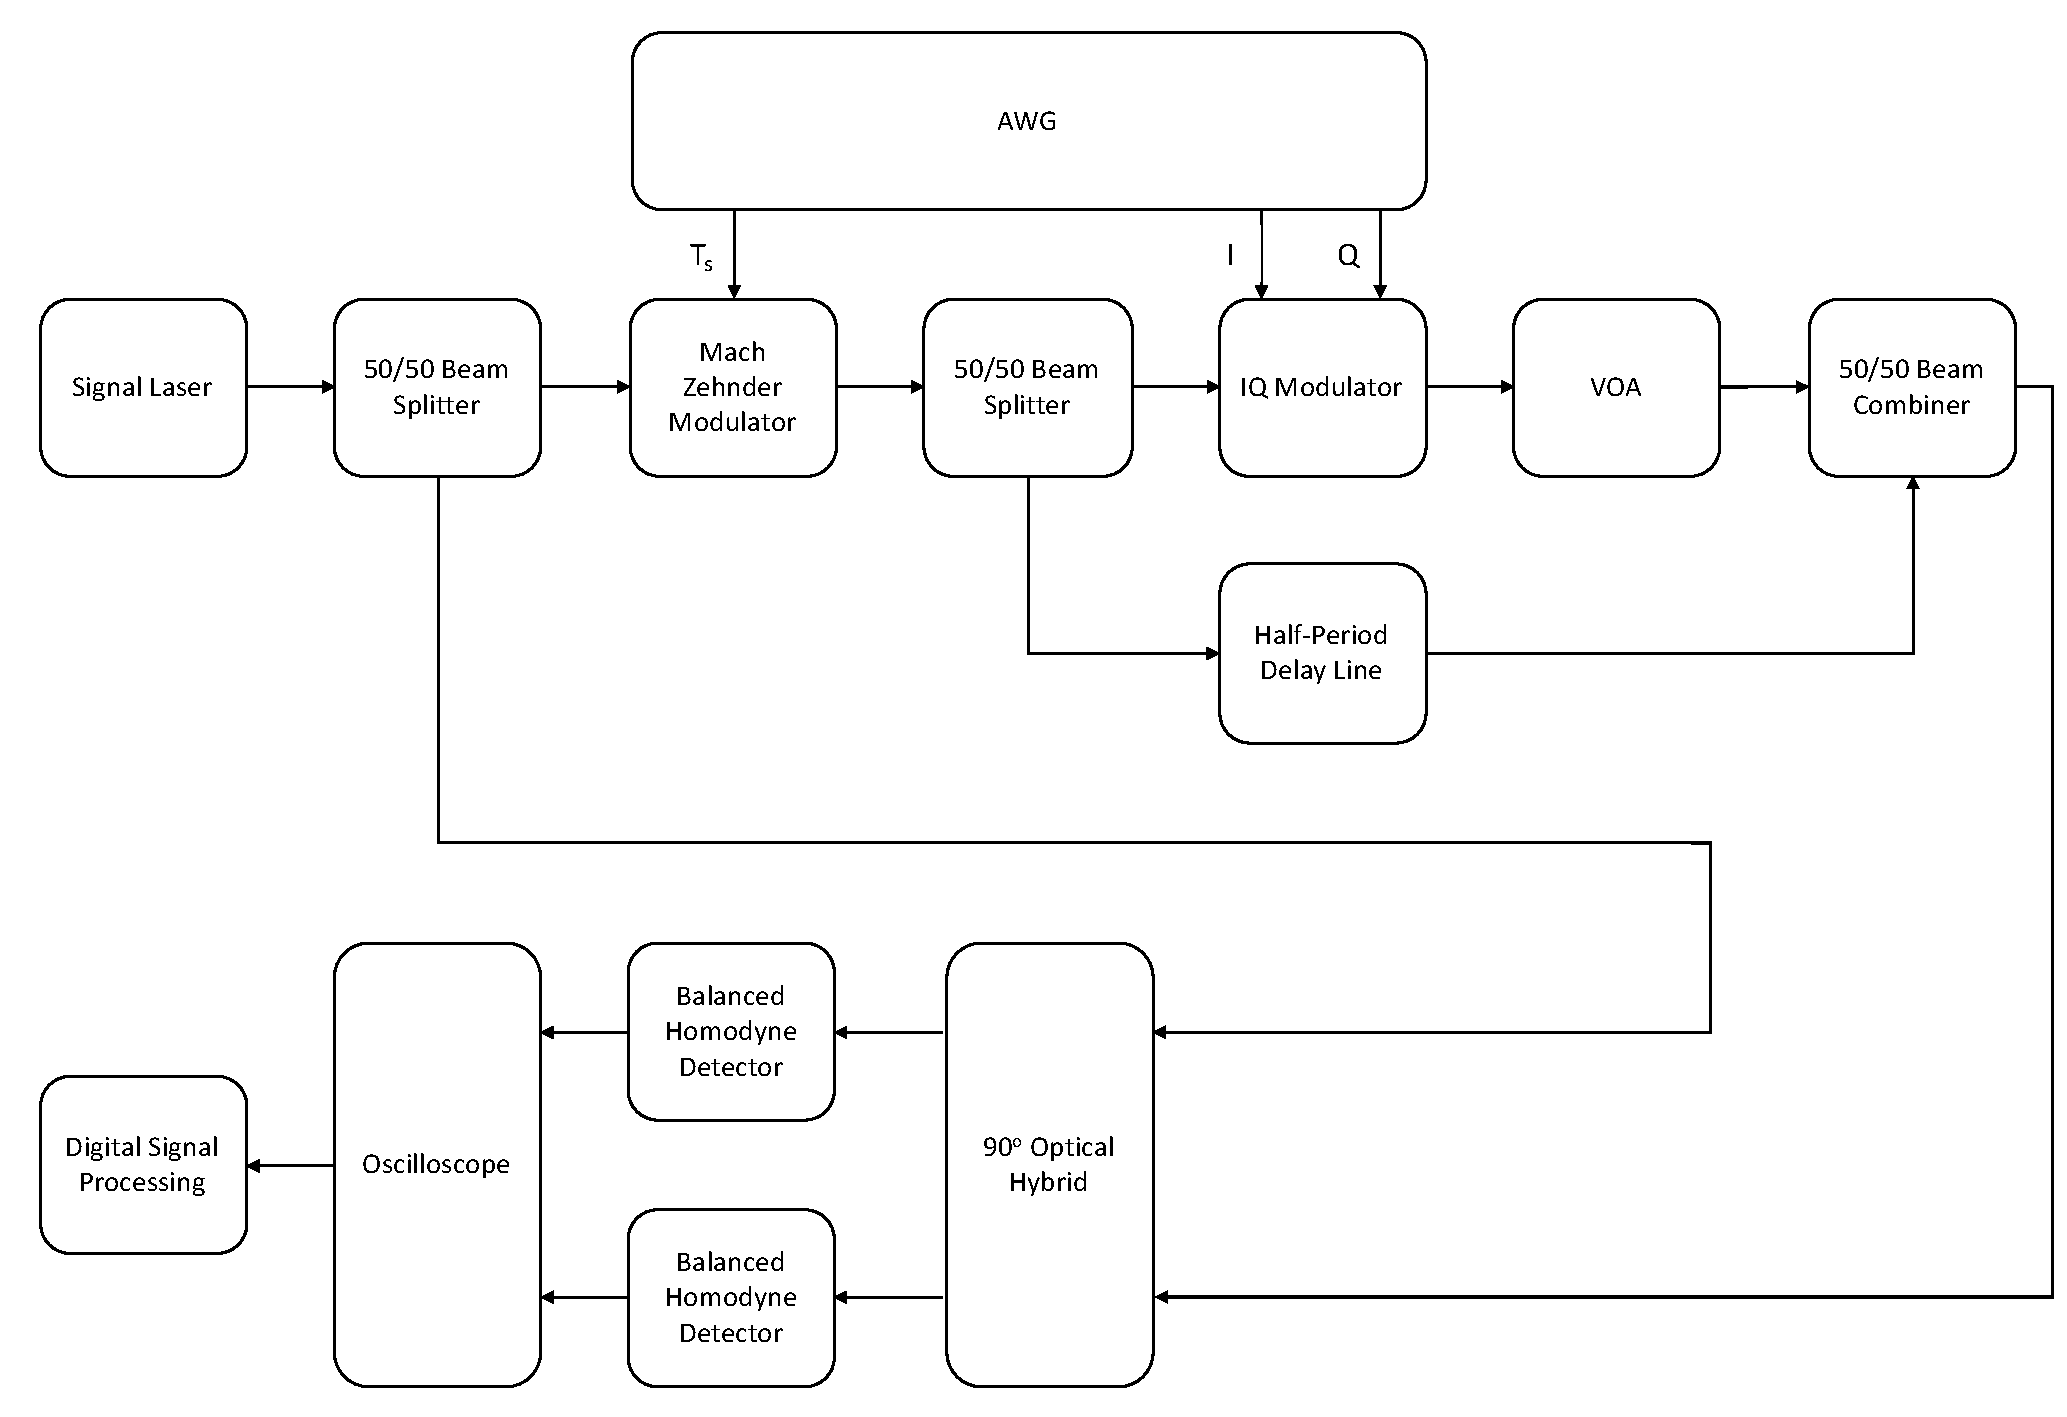
\includegraphics[width=\linewidth, trim={0cm 0cm 0cm 0cm}, clip=true]{diagram_BW_CV_EXP.pdf}
\caption{Diagram of full experimental setup.}
\label{fig:expDia}
\end{figure}
The setup contained two Yenista OSICS Band C/AG TLS lasers, tuned to a 1550~nm wavelength. A JDSU dual drive Mach-Zehnder Modulator with a Picosecond 5865 RF driver, employed at the output of one of the lasers and acting as an amplitude modulator, set the repetition rate at 1~GHz with a pulse time of 125~ps. This amplitude modulated laser is dubbed the Signal (\textbf{SI}) laser. The driving signal was generated by an Agilent Technologies BER Tester. A 50/50 beam-splitter was employed at the output of the Mach-Zehnder Modulator, one arm output is sent through an IQ Modulator while the other is sent through a fibre loop with length chosen such that the two arms have a relative delay of roughly 500~ps. The employed IQ Modulator was a u2t Photonics 32~GHz IQ Modulator with a SHF 807 RF driver, the driving signal being generated by a Tektronix AWG70002A Arbitrary Waveform Generator (\textbf{AWG}). A 15~dB attenuator followed by a Variable Optical Attenuator (\textbf{VOA}) was set at the output of the IQ modulator to allow a fine tuning of the phase modulated signal's optical power to the desired level. The two arms created by the first beam-splitter are combined by a 50/50 beam combiner. A fibre channel of $\sim10$~km was set between Alice's and Bob's setup. The second Yenista OSICS Band C/AG TLS laser, from this point dubbed the Local Oscillator (\textbf{LO}) laser, was sent through a VOA to a coherent receiver. A Picometrix CR-100D 100G Integrated Balanced Receiver for Coherent Applications with a bandwidth of  30~GHz was employed to perform double homodyne measurements, recovering both the in-phase and in-quadrature components of the incoming light field. The response of the receiver was recorded by a Tektronix DPO77002SX-R3 oscilloscope, with an acquisition frequency of 100~GHz for a period of 400~\textmu{s}.
\par
Some variations of the setup presented in Figure~\ref{fig:expDia} were used, for example using one laser instead of the two presented (adding a 50/50 beamsplitter before the Mach-Zehnder Modulator to extract the local oscillator from the same source as the signal), dubbed single laser setup, and removing the Quantum-Channel (connecting the signal generation setup directly to the detection), dubbed back to back setup. With these changes, a total of 4 setups were implemented. The objective of these changes was to reduce complexity and allow for easier identification and correction of possible errors in the experimental setup.
\par
The driving signal implemented on the AWG was generated by a short Matlab code that generated a Pseudo Random Bit Sequence (\textbf{PRBS}) with length $2^{17}$ preceded by a deterministic tram of length 32896 taking the form $1001110000(...)$.

\subsubsection{Output Data Processing}

A Matlab algorithm was developed to allow for the post-processing of the recorded experimental data. The code works as follows:
\begin{enumerate}
\item Loads the data into the Matlab workspace.
\item Generates a persistence figure isolating every information-reference pulse pair for easier post-processing (see Figure~\ref{fig:persistence1}), with the reference and signal pulses being visible, in the time ranges $\sim[0.1,0.2]\times10^{-9}~$s and $\sim[0.7,0.8]\times10^{-9}~$s respectively.
\begin{figure}[h]
\centering
\begin{subfigure}{.45\linewidth}
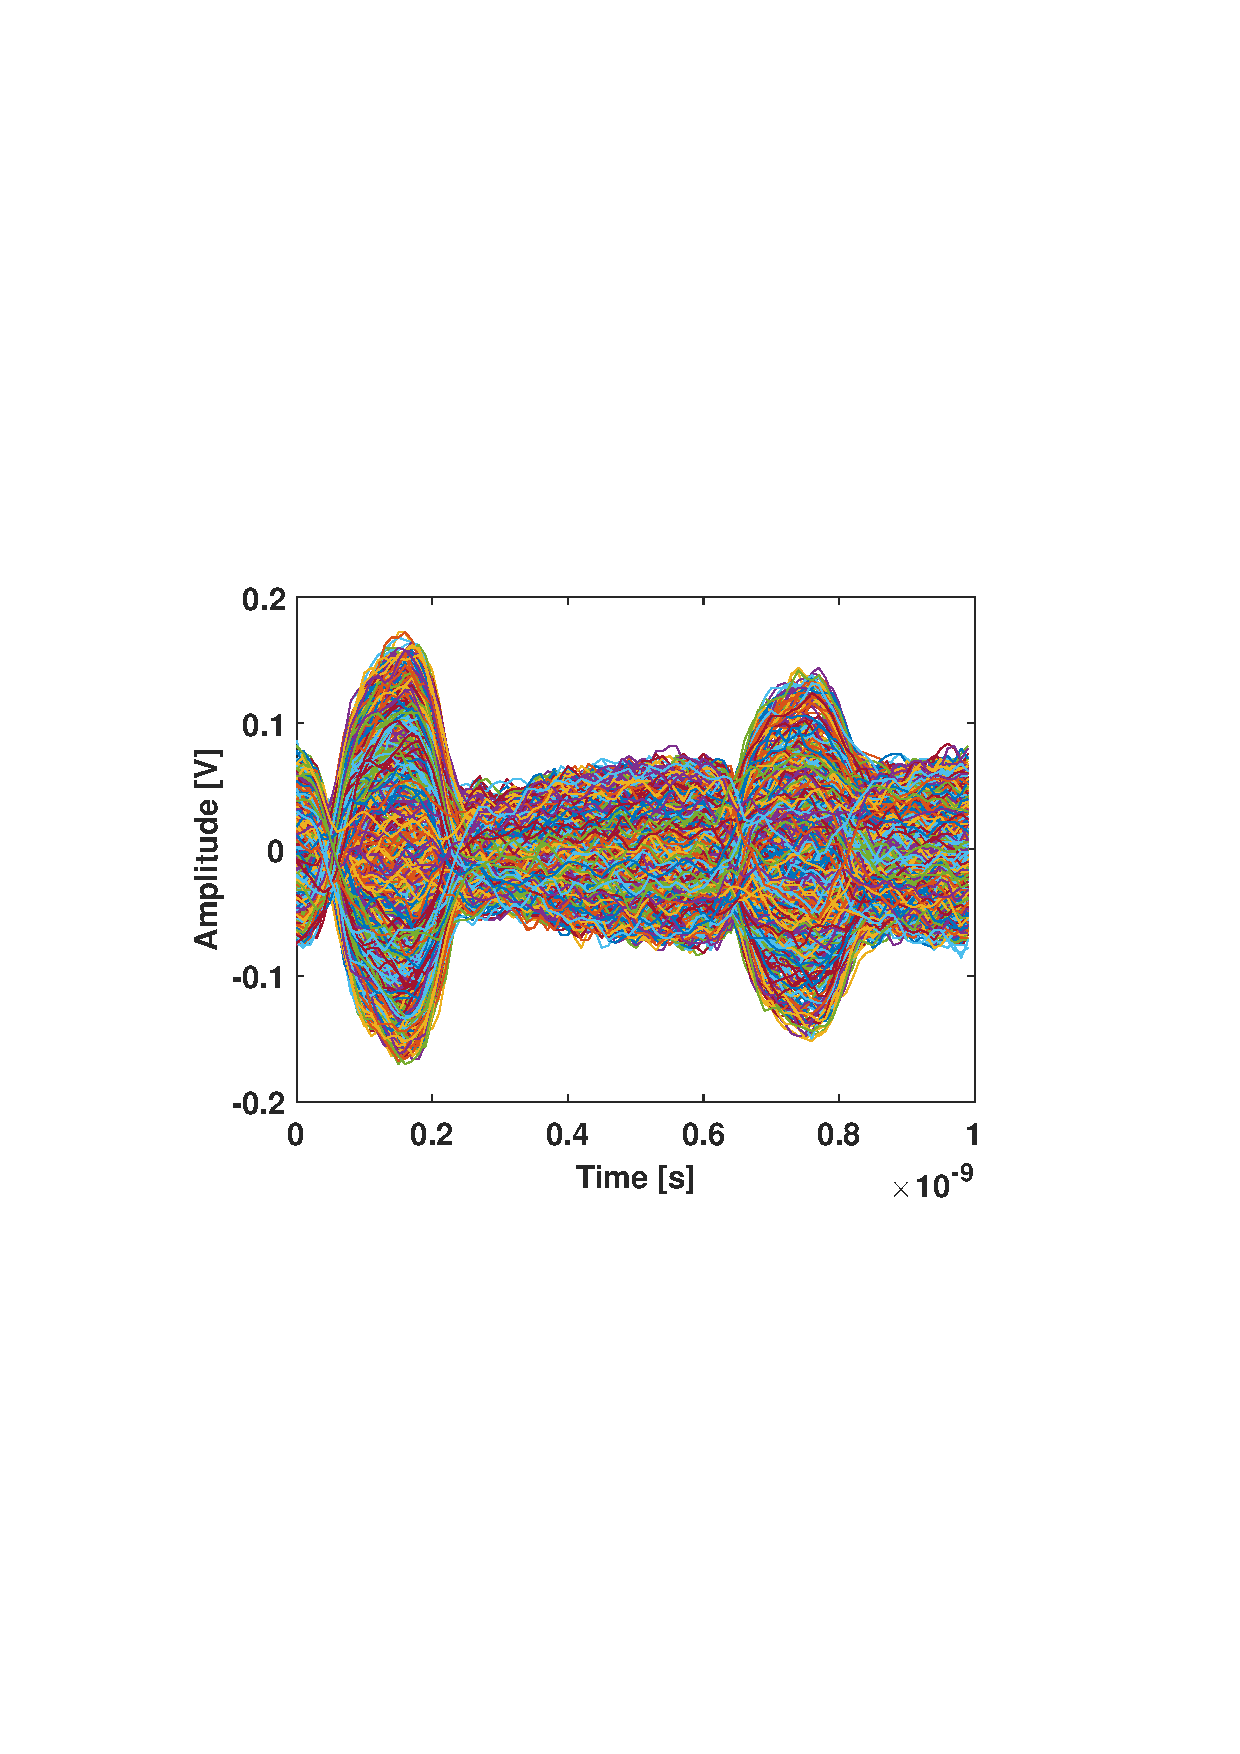
\includegraphics[width=\linewidth, trim={3cm 9cm 3cm 9.5cm}, clip=true]{persistence1.pdf}
\caption{}
\label{fig:persistence1}
\end{subfigure}
~
\begin{subfigure}{.45\linewidth}
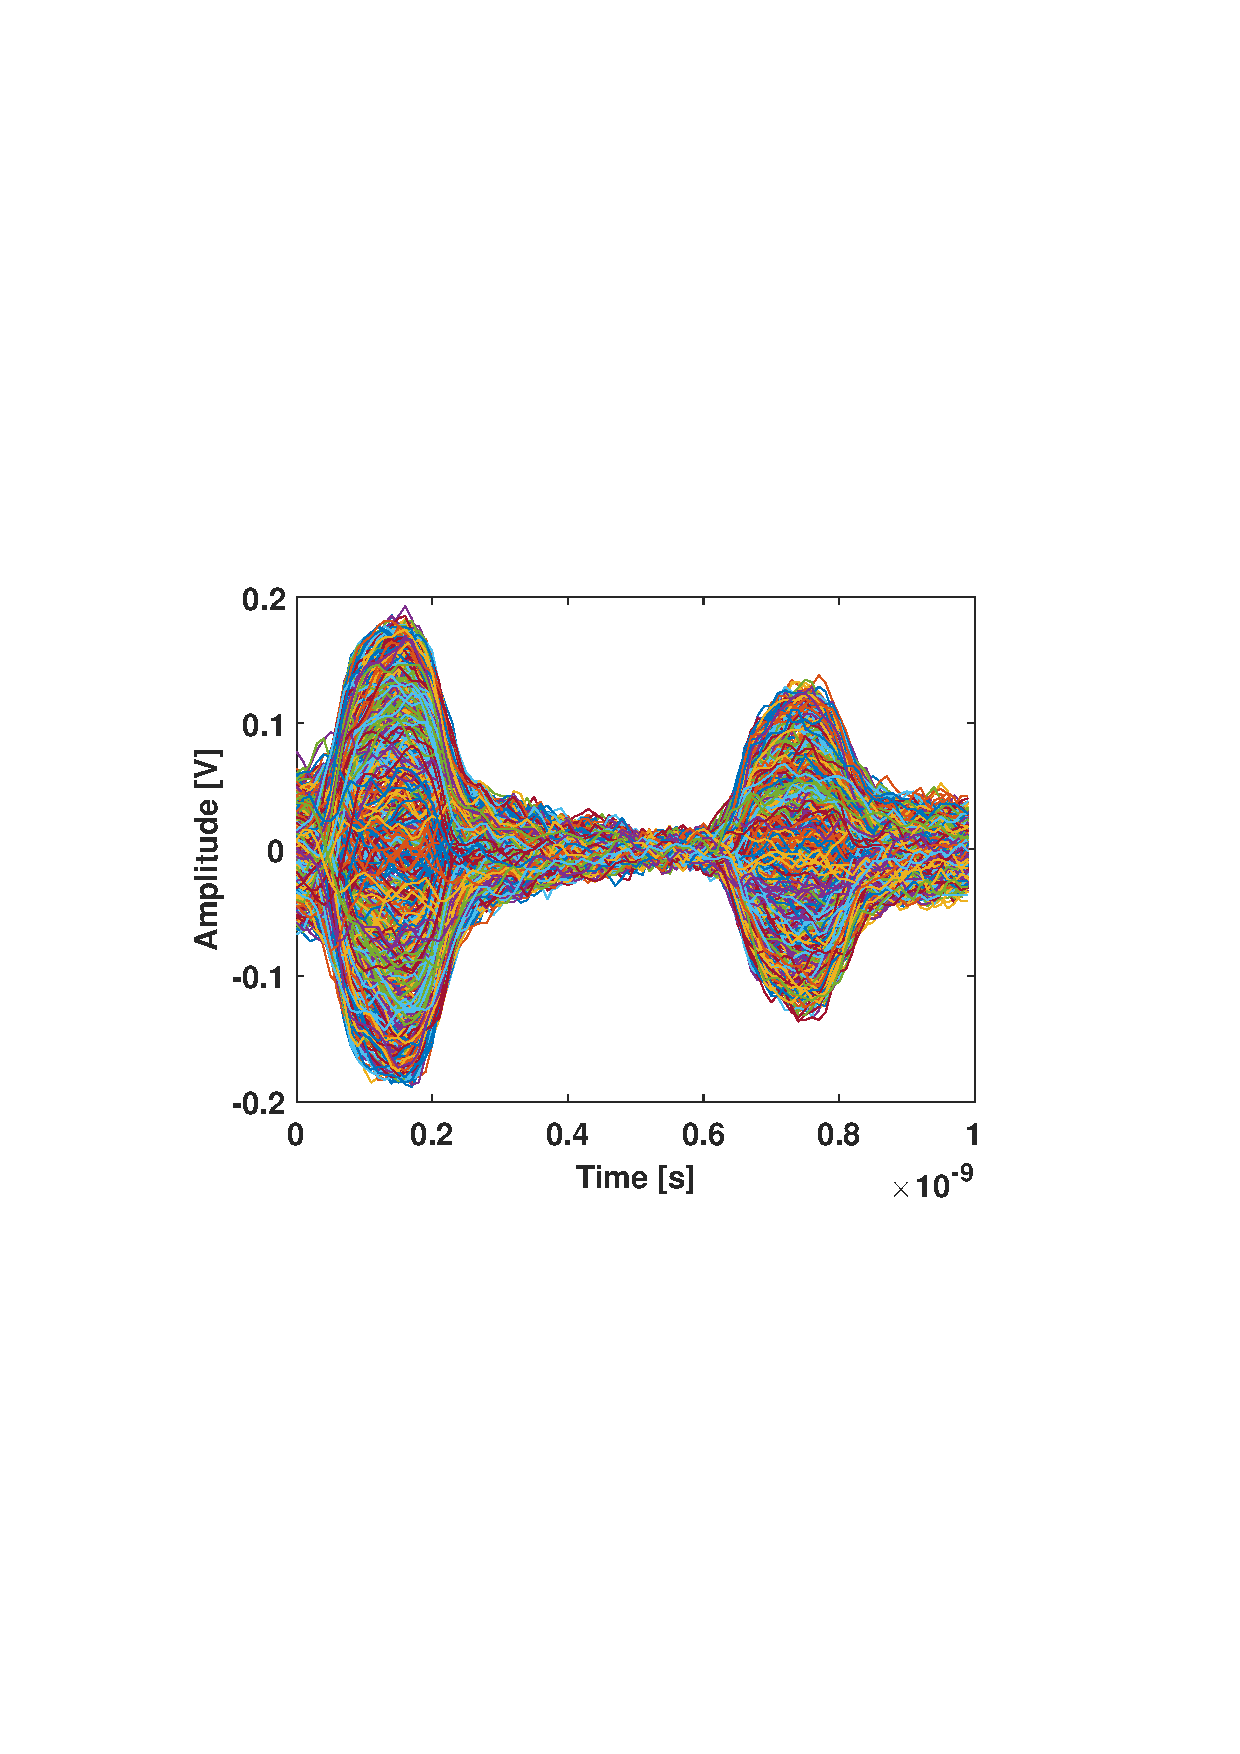
\includegraphics[width=\linewidth, trim={3cm 9cm 3cm 9.5cm}, clip=true]{persistence2.pdf}
\caption{}
\label{fig:persistence2}
\end{subfigure}
\caption{Persistence of 1000 pairs of information and reference pulses before~(a) and after~(b) low frequency noise removal.}
\label{fig:persistence}
\end{figure}
\item Removes low frequency noise by computing the average voltage value on an area outside the pulses for each persistence pair and subtracting that value from the full pair. The effect of this noise removal is noticeable in Figure~\ref{fig:persistence2}, notice the noise amplitude in the time range $\sim[0.3,0.6]\times10^{-9}~$s.
\item Selects the points inside the pulses, the following steps are performed only on these selected points.
\item Orthogonalizes the data by implementing a recursive Gram-Schmidt orthogonolazitation algorithm, adapted from the method presented in~\cite{huang2001recursive}. The correlation $r_{IQ}$ between the in-phase and in-quadrature points of the reference pulses is calculated, this correlation is then used to weigh the amount of the in-phase contribution that is subtracted from the in-quadrature element for both the signal and reference pulses. For $i\geq2$ this algorithm takes the form:
\begin{equation}
\begin{cases}
r_{IQ}(i)=r_{IQ}(i-1)+p\left(\text{Q}_r(i-1)\text{I}_r(i-1)-r_{IQ}(i-1)\right)\\
\text{Q}_{ro}(i)=\text{Q}_r(i)-r_{IQ}(i)\text{I}_r(i)\\
\text{Q}_{so}(i)=\text{Q}_s(i)-r_{IQ}(i)\text{I}_s(i)\\
\end{cases},
\end{equation}
with I$_r$/I$_s$ being the in-phase components of the reference/signal pulses, which are maintained, Q$_{r}$/Q$_{s}$ are the initial in-quadrature components of the reference/signal pulses, while Q$_{ro}$/Q$_{so}$ are the in-quadrature components of the of the reference/signal pulses after removal of the in-phase contribution. For $i=1$, $r_{IQ}$ was set at 0 and $p$ is a small number that we have chosen to be $10^{-3}$. The effect of this orthogonalization procedure is presented graphically in Figure~\ref{fig:orthogonalization}.
\begin{figure}[h]
\centering
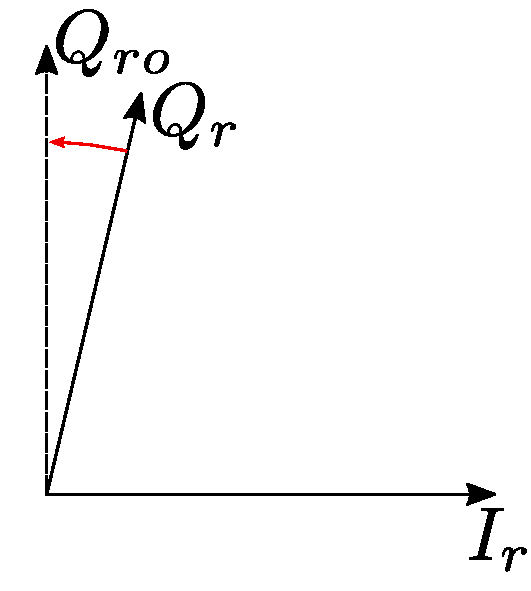
\includegraphics[width=.2\linewidth]{orthogonalization.pdf}
\caption{Visual representation of the employed axis orthogonalization.}
\label{fig:orthogonalization}
\end{figure}
This algorithm is applied on the reference pulses. Before this step the constellation consists of an ellipse with a small eccentricity, while after application of the algorithm the constellation becomes a circle, removing the detector imbalances. This algorithm is implemented only on the reference pulses because of the extremely low Signal to Noise Ratio (\textbf{SNR}) of the signal pulses while working at quantum levels. This algorithm has a short convergence time, rendering the first bits (numbering roughly $10^4$) unusable.
\item Removes the phase difference between the signal and local oscillator lasers, see Figure~\ref{fig:driftCompens}, where it is clear that the constellation presented in Figure~\ref{fig:phasedriftA} is a dragging rotation of the constellation in Figure~\ref{fig:phasedriftB}. The compensation of the phase difference between the signal and local oscillator is accomplished by measuring the phase of the reference pulses in relation to the local oscillator, this phase difference is then subtracted from the phase measured from the signal pulses. This is accomplished by multiplying the signal constellation with the conjugate of the normalized reference constellation. It is visible that the constellation before the phase drift compensation is a dragging rotation of the QPSK constellation obtained afterwards.
\begin{figure}[h]
\centering
\begin{subfigure}{.45\linewidth}
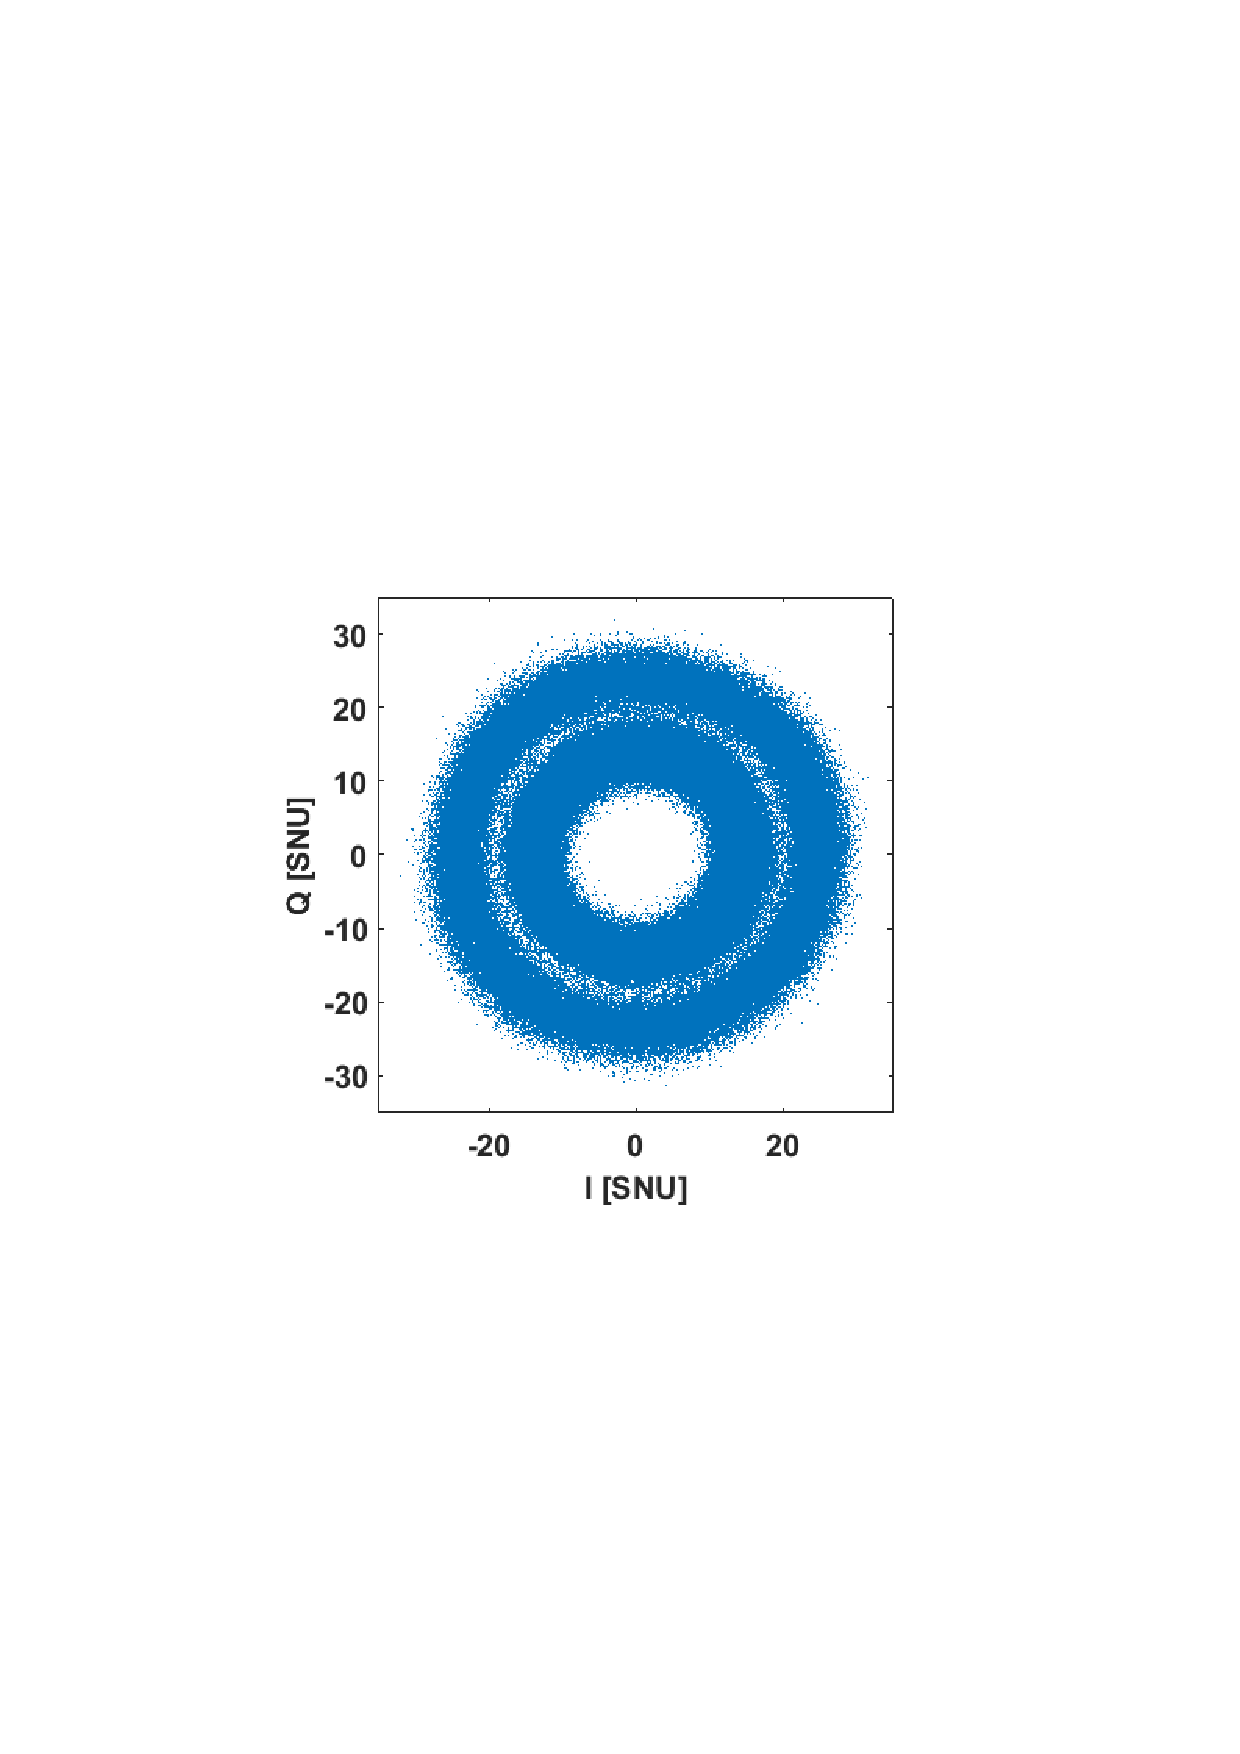
\includegraphics[width=\linewidth, trim={3cm 9cm 3cm 9.5cm}, clip=true]{doubleBTBSNUBefPhasDriftComp.pdf}
\caption{}
\label{fig:phasedriftA}
\end{subfigure}
~
\begin{subfigure}{.45\linewidth}
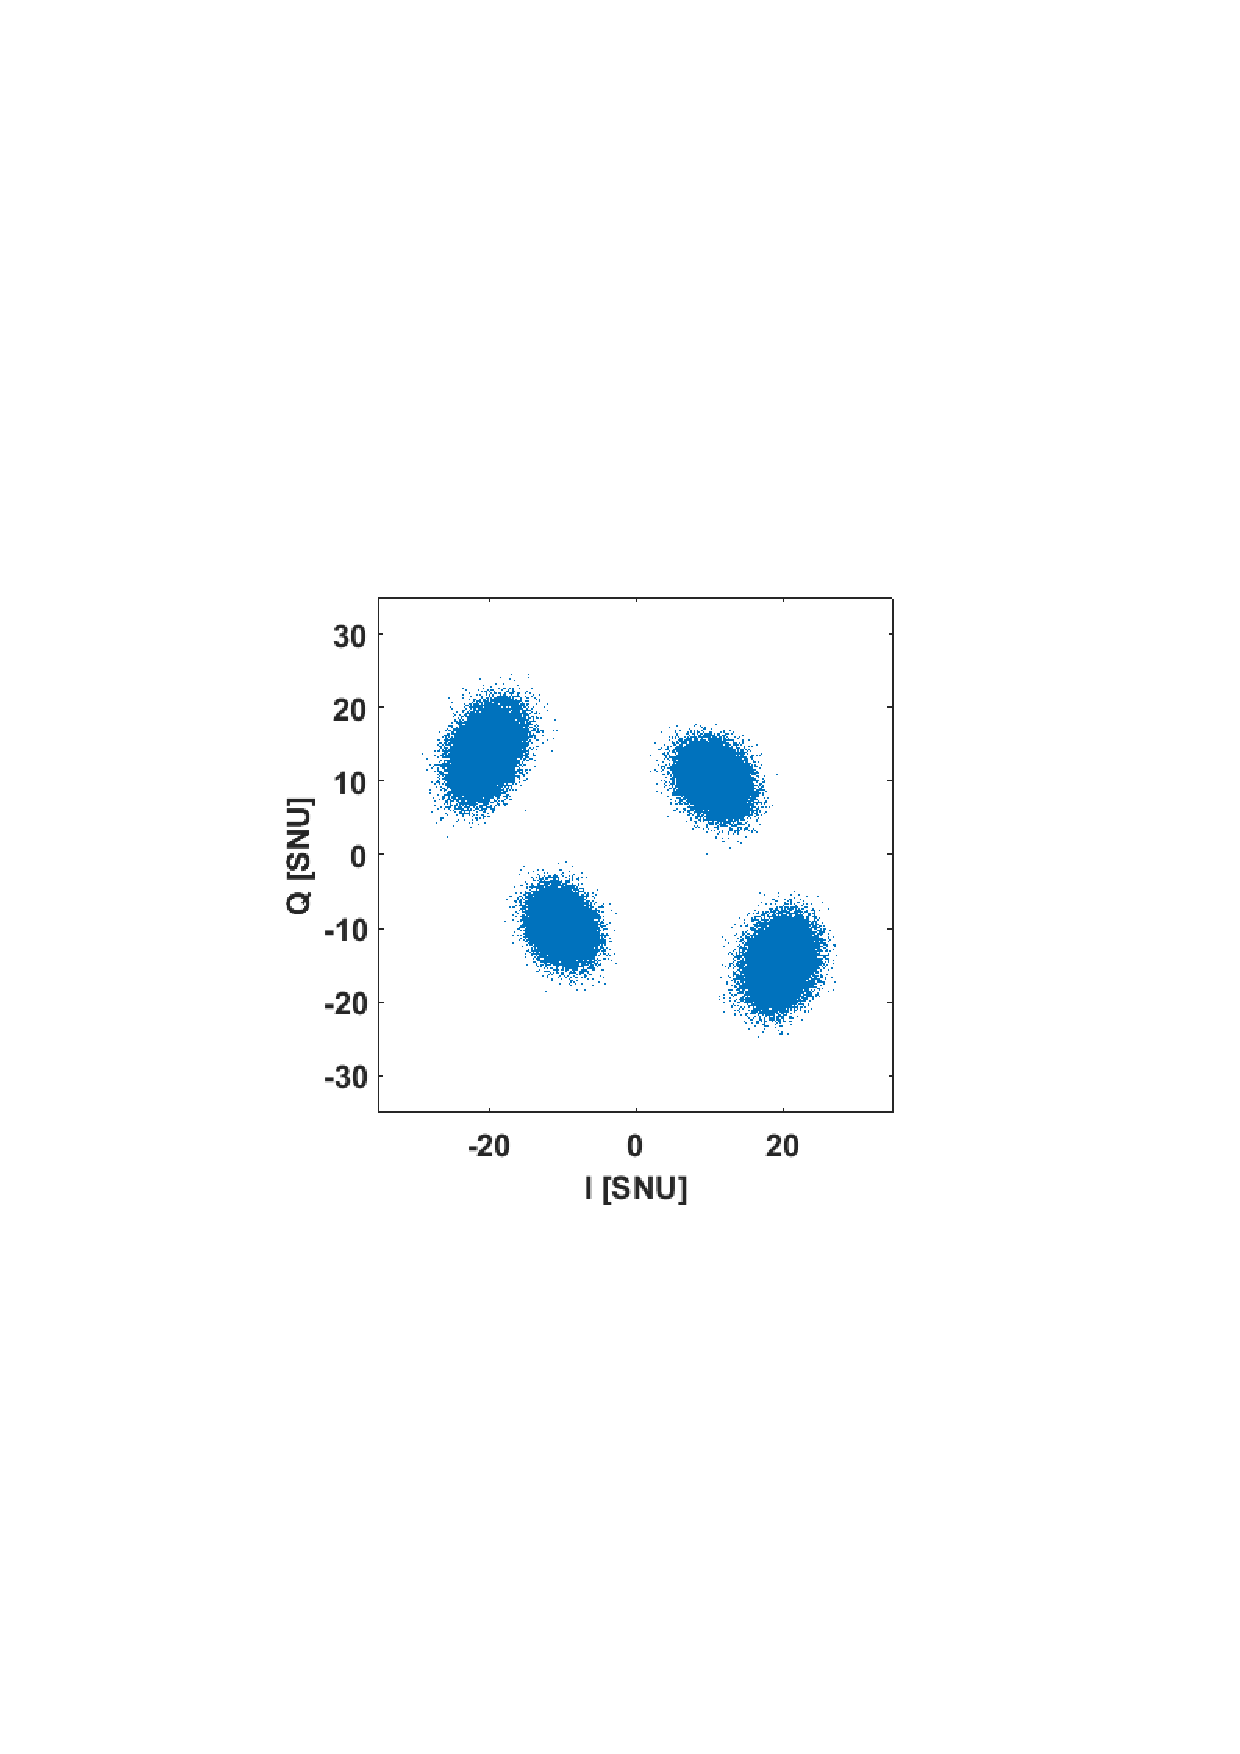
\includegraphics[width=\linewidth, trim={3cm 9cm 3cm 9.5cm}, clip=true]{doubleBTBSNU.pdf}
\caption{}
\label{fig:phasedriftB}
\end{subfigure}
\caption{Signal constellation before (a) and after (b) phase difference compensation.}
\label{fig:driftCompens}
\end{figure}
\item Ranges the start of the PRBS sequence via detection of the deterministic tram mentioned above.
\item Corrects rotations of the constellation via minimization of the error of the deterministic tram. Given the laser's central frequency fluctuations, this rotation should be compensated at regular intervals during transmission.
\item Converts the signal constellation to shot noise units.
\item Estimates the secret key rate obtained from the recovered bit string.
\end{enumerate}
\par
Figure~\ref{fig:recConst} presents the recovered constellations for single and double laser setups at high levels of signal power ($\sim$200 photons per pulse on average). The expected output would be a \textit{square} four state constellation, while the observed results show a clear skew on the recovered constellation. We conclude this is due to imbalances on the modulation stage, this is the reason why this imbalance appears in both the single and double laser schemes. These imbalances are to be expected and in classical communications they would be compensated by applying an orthogonalization method on the data, this is not an option for our setup because at quantum levels the signal to noise ratio is so low that such methods are not efficient.
%COMMENT THE BER AND THE CONSTELLATION SKEW, PIVOT TO QUANTUM LEVEL AND SAY WE NEED TO START BY PERFORMING SHOT NOISE CHARACTERIZATION.
\begin{figure}[h]
\centering
\begin{subfigure}{.45\linewidth}
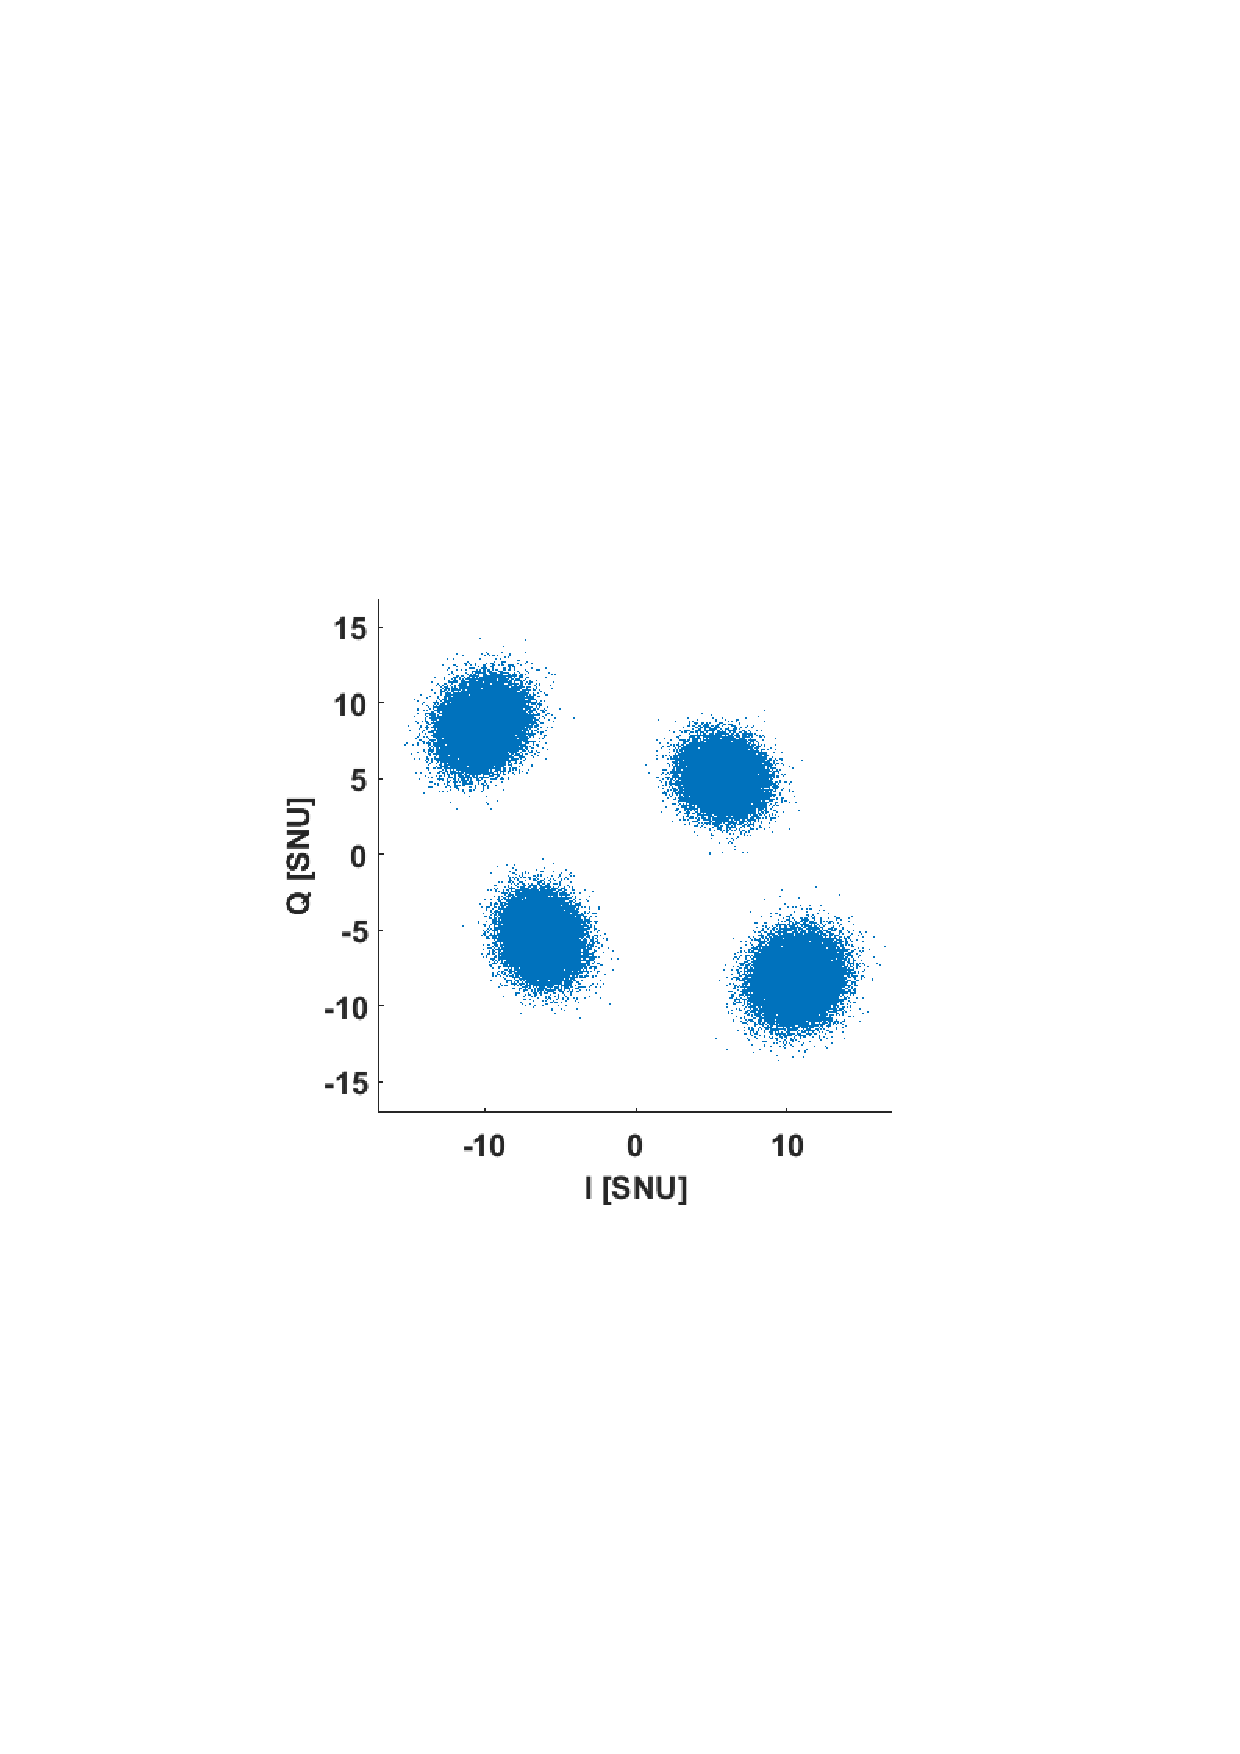
\includegraphics[width=\linewidth, trim={3cm 9cm 3cm 9.5cm}, clip=true]{singleBTBSNU.pdf}
\caption{}
\end{subfigure}
~
\begin{subfigure}{.45\linewidth}
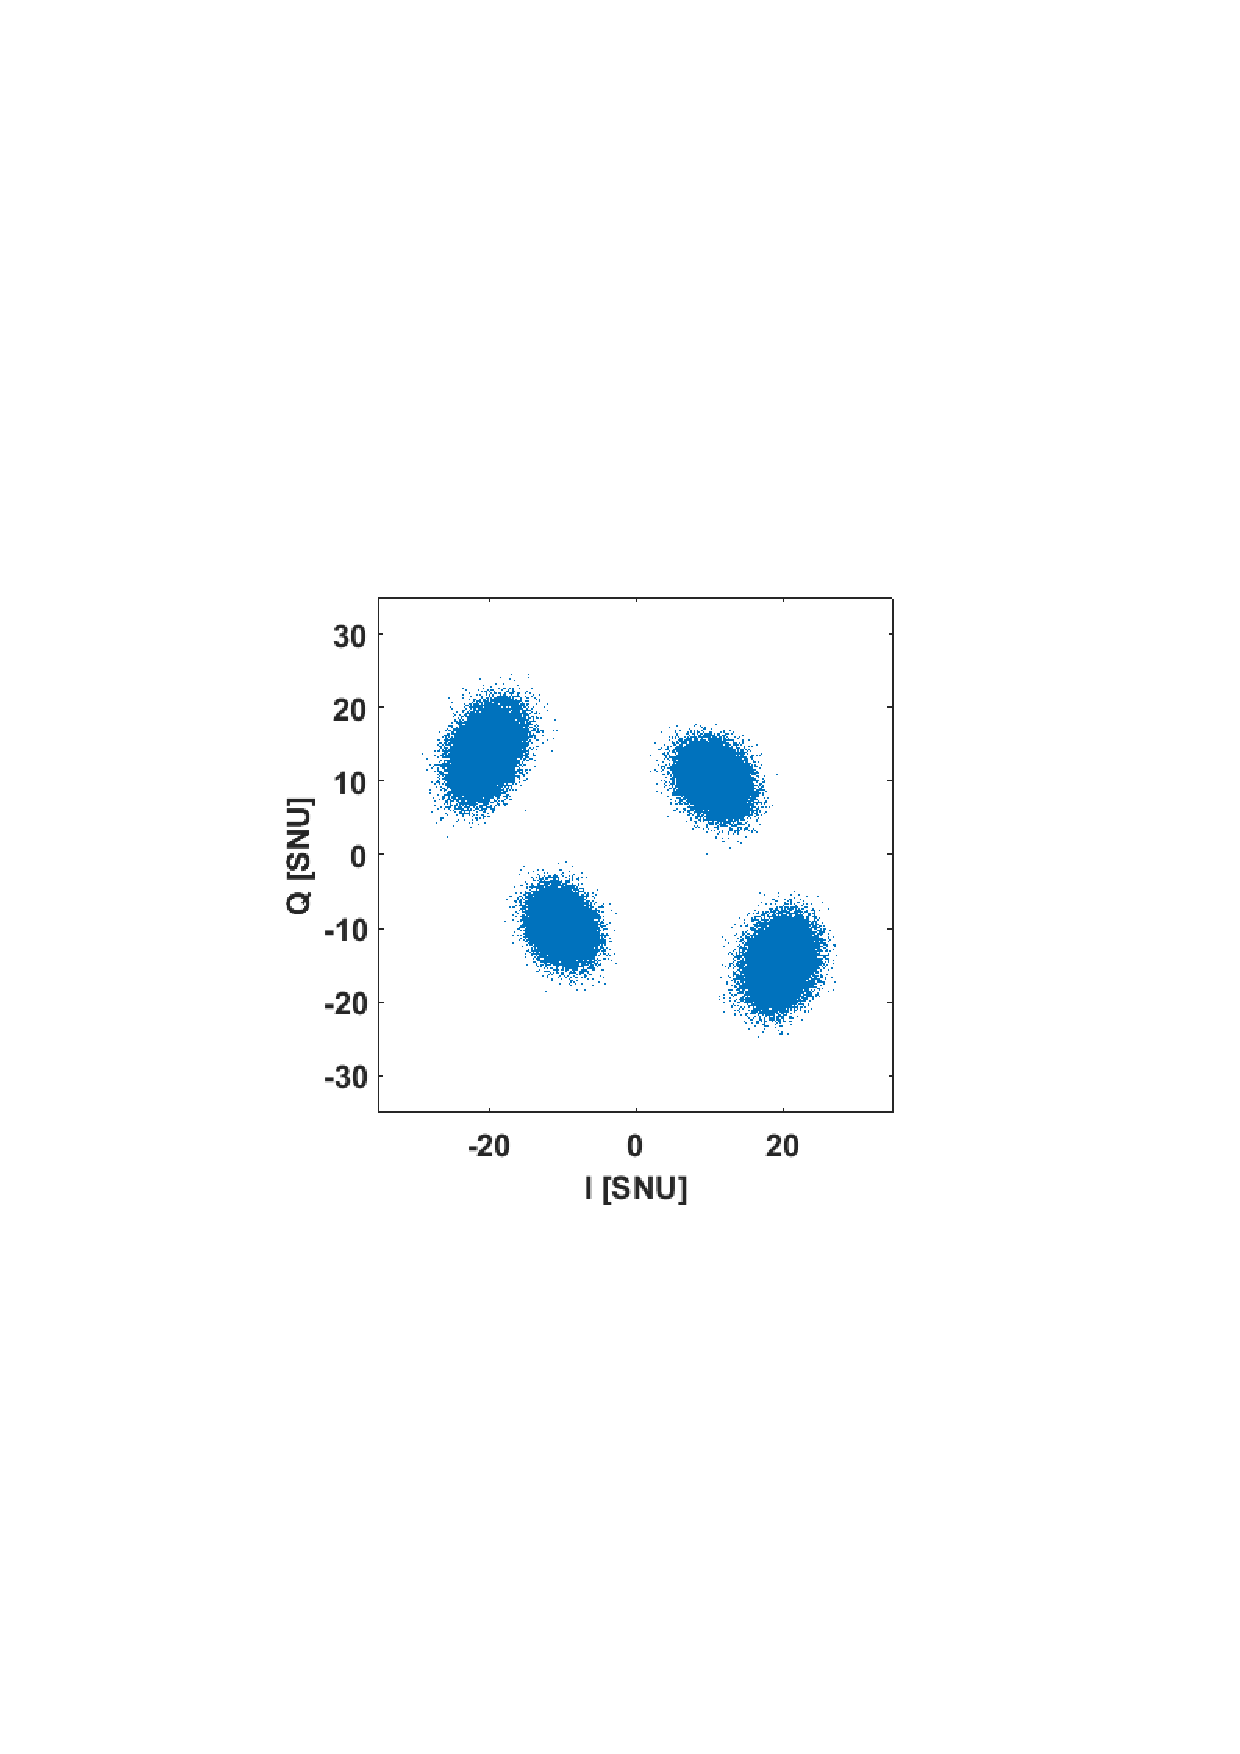
\includegraphics[width=\linewidth, trim={3cm 9cm 3cm 9.5cm}, clip=true]{doubleBTBSNU.pdf}
\caption{}
\end{subfigure}
\caption{Final constellation for single (a) and double (b) laser setups.}
\label{fig:recConst}
\end{figure}

\subsection{Comparative Analysis}

\bibliographystyle{unsrt}
 
\bibliography{bibliography}
